\documentclass{beamer}

\mode<presentation>{
	\usetheme{Boadilla}
}

%Packages
\usepackage[utf8]{inputenc}
\usepackage[ngerman]{babel}
\usepackage{graphicx}
\usepackage{booktabs}
\usepackage{mathtools}
\usepackage{amsmath}
\usepackage{listings}
\usepackage[utf8]{inputenc}
\usepackage[ngerman]{babel}
\usepackage[T1]{fontenc}
\usepackage{lmodern}
\usepackage{tabto}
\usepackage{listings}

%Einstellungen der Präsentation
\title[Social Engineering]{Soziotechnische Lösungsänsätze für Phishing Angriffe }
\author{Moritz Rupp}
\institute[MR]{Hochschule Albstadt-Sigmaringen}

\date{SS 23}


\begin{document}
\begin{frame}
 \titlepage
\end{frame}
\begin{frame}
 \frametitle{Inhalt}
 \tableofcontents
\end{frame}
\section{Was ist ein Soziotechnisches System?}
\begin{frame}{Was ist ein Soziotechnisches System? }
 \frametitle{Was ist ein Soziotechnisches System}
 ``Unter einem soziotechnischen System versteht man eine organisierte Menge von Menschen und mit diesen verknüpfte Technologien, welche in einer bestimmten Weise strukturiert sind, um ein spezifisches Ergebnis zu produzieren.''\\
 – Günter Ropohl 2009
 \\
 \vspace{10mm}
 Ein Soziotechnisches System besteht aus 2 Grund-Komponenten
 \begin{itemize}
  \item Technische Teilkomponente - Computer, Maschiene
  \item Soziale Teilkomponente - Mitarbeiter
 \end{itemize}
\end{frame}
\begin{frame}
\begin{center}
 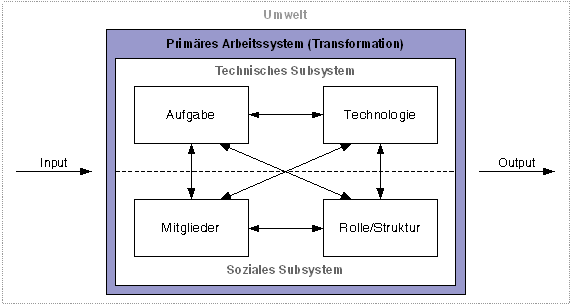
\includegraphics[scale=0.5]{data/sozio.png}

\end{center}

\end{frame}
\section{Systemtheoretische Betrachtungen}
\begin{frame}{Systemtheoretische Betrachtungen}
- Beschreibung der Abhängigkeit von sozialen und Technischen Systeme.\\
\vspace{2mm}
 \frametitle{Systemtheoretische Betrachtungen}
 „Ein Computer wird erst wirklicher Computer, wenn er zum Teil einer Mensch-Maschine-Einheit geworden ist. Wenn Text geschrieben wird, tut das nicht allein der Mensch, aber es ist auch nicht allein der Computer, der den Text schreibt; erst die Arbeitseinheit von Mensch und Computer bringt die Textverarbeitung zuwege“
 
 – Günter Ropohl 2009
\end{frame}
\section{Anwendung auf Phishing Methoden}
\begin{frame}{Anwendung auf Phishing Methoden}
 \frametitle{Anwendung auf Phishing Methoden}
 
 \begin{itemize}
  \item Phishing bedient sich Soziotechnischen Methoden
  \item Kombination von technischen und sozialen Systemen
 \end{itemize}

\end{frame}
\section{Konkret technische Lösungen}
\begin{frame}{Konkrete Technische Lösungen}
 \frametitle{Konkrete Technische Lösungen}
 \begin{itemize}
  \item DNS-Header - SPF, DMARC etc.
  \item Container Lösungen
 \end{itemize}

\end{frame}


\end{document}
